\section{Modello di Sviluppo}
\label{ModelloSviluppo}

Dopo un'attenta analisi dei vari modelli di sviluppo, considerando le caratteristiche del prodotto finale che deve essere sviluppato, abbiamo  scelto di utilizzare il modello di tipo incrementale. Il gruppo ha valutato che la relativa semplicità nell'identificare insiemi di funzionalità di importanza massima, con consguenti funzionalità di importanza più marginale, ben si sposasse con la natura del modello incrementale.

\subsection{Modello Incrementale}

\begin{figure}[h]
	\centering
  		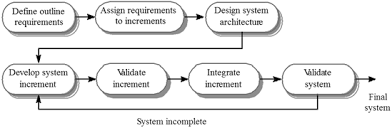
\includegraphics[width=0.7\linewidth]{./images/modelloincrementale.png}
  		\caption{Modello Incrementale da : \url{https://www.math.unipd.it/~tullio/IS-1/2015/Dispense/L03.pdf} slide numero 18}
  		\label{fig:Modello Incrementale}
\end{figure}

Il modello incrementale prevede rilasci multipli e successivi del prodotto ed ogni rilascio prevede un incremento delle sue funzionalità. \\
Con questo modello vengono pianificati quanti incrementi verranno effettuati basandosi sui requisiti obbligatori ed opzionali richiesti dalla proponente, aggiungendovi delle priorità di sviluppo in modo tale che elementi con priorità maggiore vengano sviluppati prima di elementi con priorità minore.\\
Il prodotto finale non sarà rilasciato nella sua completezza in un solo momento ma prevederà, appunto, degli incrementi. \\
È fondamentale decidere i requisiti con completezza prima di iniziare lo sviluppo dell'attuale incremento, mentre requisiti aggiuntivi per incrementi futuri sono adeguati. Per ogni sviluppo delle parti è necessario analizzare il suo grado di efficacia\glossario prima di integrare le parti tra di loro. Terminato l'incremento attuale si andrà avanti con l'incremento successivo scelto precedentemente, qualora il prodotto non sia completo. \\
Il vantaggio di utilizzare questo modello racchiude, tra le varie, un rilascio delle funzionalità base nei primi incrementi, il che comporta una maggiore verifica e quindi una maggiore stabilità. Oltretutto i primi incrementi possono derivare da una prototipazione, la quale aiuta a fissare meglio i requisiti per gli elementi successivi. Un ulteriore vantaggio è la riduzione del rischio di fallimento, senza azzerarlo in quanto costi aggiuntivi posso derivare dalla caduta nell'iterazione\glossario.

\subsubsection{Incremento}\label{inc}
Un incremento è composto dalle seguenti fasi:
\begin{itemize}
	\item Assegnazione dei task ai componenti del gruppo;
	\item Completamento dei task;
	\item Verifica e valutazione del prodotto.
\end{itemize}
Gli incrementi dovranno rispettare i periodi descritti nel capitolo seguente.\\
Il gruppo prevede di effettuare tre incrementi durante la fase di codifica, con conseguente consegna alla proponente di due prototipi del prodotto, più un ulteriore incremento finale durante la fase precedente alla consegna, a scopo di raffinare quanto già prodotto.
Il gruppo si impegna a consegnare i due prototipi entro le seguenti date:

\begin{itemize}
	\item \textbf{Primo Prototipo}: 1 Marzo 2019\\
	Questo primo prototipo fungerà da dimostrazione tangibile del buon funzionamento del prodotto, a supporto
	delle scelte di progettazione fatte. Il gruppo ha valutato che fornire un monitoraggio dei dati funzionante fosse la funzionalità basilare dell'intero prodotto, ed ha dunque deciso di progettare in tal senso il primo incremento. Il prototipo dovrà, come requisiti minimi fissati dal gruppo, implementare le seguenti funzionalità:
	\begin{enumerate}	% TODO: Inserire il riferimento ai requisiti coinvoliti
		\item Consentire la comunicazione con le \textit{Grafana API}\glossario per poter ottenere le sorgenti dati disponibili;
		\item Consentire il reperimento dati da \textit{InfluxDB}\glossario;
		\item Caricamento di una rete bayesiana;
		\item Interpretazione della rete bayesiana caricata;
		\item Collegamento dei nodi;
		\item Impostazione di una politica temporale per il ricalcolo delle probabilità
		\item Consentire che il monitoraggio dati sia avviabile, e che quindi siano visibili i valori di probabilità calcolati ciclicamente in base a quanto definito nella politica temporale.
	\end{enumerate}
	
	\item \textbf{Secondo Prototipo}: 10 Aprile 2019\\
	Il secondo prototipo dovrà dimostrare di essersi evoluto a partire dal prototipo precedente, riportando le correzioni suggerite dalla proponente. Questo secondo incremento ha come obiettivo principale consentire un monitoraggio continuo dei dati, indipendente dal browser. Nello specifico il prototipo dovrà implementare le seguenti funzionalità, fissate dal gruppo:
	\begin{enumerate} % TODO: Inserire il riferimento ai requisiti coinvoliti
		\item Introdurre un server che consenta di mantenere la consistenza dei dati anche a browser\glossario chiuso;
		\item Collegamento al server;
		\item Consolidamento delle funzionalità precedenti, in particolare sviluppo del front-end;
		\item Possibilità di monitorare più reti;
		\item Possibilità di salvare le reti caricate ed eliminarle;
		\item Possibilità di interrompere il monitoraggio;
		\item Possibilità di scollegare nodi precedentemente collegati;
		\item Separazione tra vista di impostazione e vista di monitoraggio.
	\end{enumerate}

\end{itemize}

Oltre ai prototipi è prevista la consegna del prodotto finale, raffinato a partire dall'ultimo prototipo, durante l'ultimo incremento:
\begin{itemize}
	\item \textbf{Prodotto finale}: 17 Maggio 2019\\
	La consegna di tale ultimo incremento dovrà includere correzioni segnalate alla consegna del prototipo precedente. Inoltre, l'aspetto grafico verrà perfezionato ulteriormente portando tale componente ad un livello considerabile come definitivo. Le funzionalità che devono essere implementate in questo ultimo incremento sono di natura opzionale, ma forniscono un notevole valore aggiunto al prodotto finale. Queste sono:
	\begin{enumerate}
		\item Introduzione di una impostazione, in fase di collegamento dei nodi, che permetta di ignorare la politica temporale al verificarsi dell'evento;
		\item Visualizzazione dei dati di monitoraggio sotto forma di rappresentazione grafica delle rete bayesiana monitorata, anziche semplice forma tabellare.
	\end{enumerate}
\end{itemize}



